\section{Referencia del Archivo /media/docs/progra/c++/compiladores1/proy2/godzilla/src/symtab.c}
\label{symtab_8c}\index{/media/docs/progra/c++/compiladores1/proy2/godzilla/src/symtab.c@{/media/docs/progra/c++/compiladores1/proy2/godzilla/src/symtab.c}}
Implementacion de la tabla de simbolos.Incluye la implementacion de rutinas de insercion, busqueda y eliminacion. 

{\tt \#include $<$stdio.h$>$}\par
{\tt \#include $<$stdlib.h$>$}\par
{\tt \#include $<$string.h$>$}\par
{\tt \#include \char`\"{}symtab.h\char`\"{}}\par
{\tt \#include \char`\"{}constantes.h\char`\"{}}\par


Dependencia gr\'{a}fica adjunta para symtab.c:\begin{figure}[H]
\begin{center}
\leavevmode
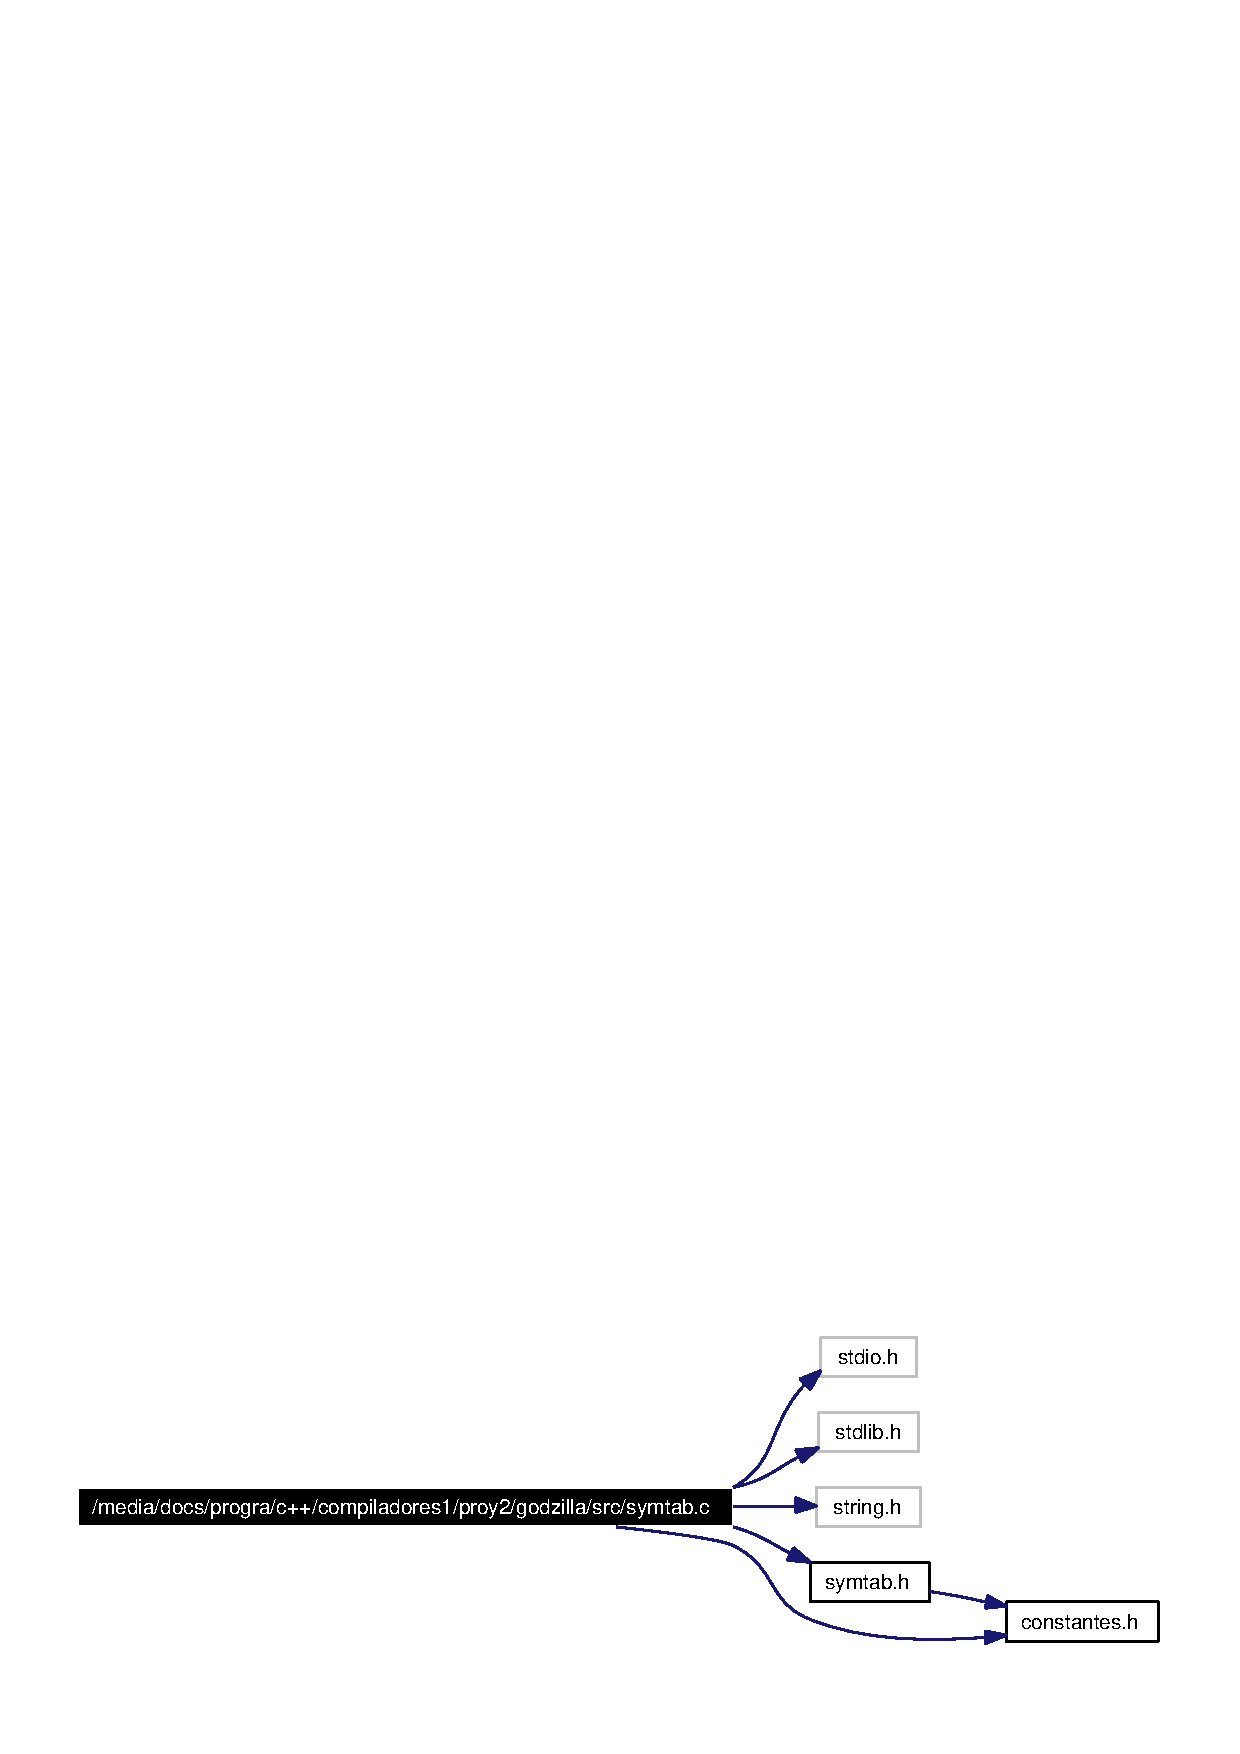
\includegraphics[width=278pt]{symtab_8c__incl}
\end{center}
\end{figure}
\subsection*{Funciones}
\begin{CompactItemize}
\item 
{\bf symbol} $\ast$ {\bf insertar\-Simbolo} (char $\ast$id, int tipo)
\begin{CompactList}\small\item\em Inserta un nuevo simbolo sin comprobar su previa existencia. \item\end{CompactList}\item 
{\bf symbol} $\ast$ {\bf buscar\-Simbolo} (char $\ast$id)
\begin{CompactList}\small\item\em Busca y devuelve simbolo segun su identificador dado en el param. \item\end{CompactList}\item 
void {\bf borrar\-Nodos} ({\bf symbol} $\ast$s)
\item 
void {\bf borrar\-Tabla} ()
\begin{CompactList}\small\item\em Elimina todos los registros de la tabla de simbolos. \item\end{CompactList}\item 
int {\bf open\-Symtab\-File} (const char $\ast$filename)
\begin{CompactList}\small\item\em Abre archivo hacia donde se imprimira archivo de tabla de simbolos. \item\end{CompactList}\item 
int {\bf close\-Symtab\-File} ()
\begin{CompactList}\small\item\em Cierra archivo hacia donde se escribio tabla de simbolos. \item\end{CompactList}\item 
int {\bf print\-Symtab\-File} (int linea)
\begin{CompactList}\small\item\em Imprime tabla de simbolos a archivo dado. \item\end{CompactList}\end{CompactItemize}
\subsection*{Variables}
\begin{CompactItemize}
\item 
static {\bf symtab} {\bf tabla}
\item 
static FILE $\ast$ {\bf symtabfile} = NULL
\begin{CompactList}\small\item\em Tabla de simbolos. \item\end{CompactList}\end{CompactItemize}


\subsection{Descripci\'{o}n detallada}
Implementacion de la tabla de simbolos.Incluye la implementacion de rutinas de insercion, busqueda y eliminacion. 



Definici\'{o}n en el archivo {\bf symtab.c}.

\subsection{Documentaci\'{o}n de las funciones}
\index{symtab.c@{symtab.c}!borrarNodos@{borrarNodos}}
\index{borrarNodos@{borrarNodos}!symtab.c@{symtab.c}}
\subsubsection{\setlength{\rightskip}{0pt plus 5cm}void borrar\-Nodos ({\bf symbol} $\ast$ {\em s})}\label{symtab_8c_a4}


No usar free() da error SIGABRT 

Definici\'{o}n en la l\'{\i}nea 74 del archivo symtab.c.

Hace referencia a symbol::id, symbol::siguiente, T\_\-STRING, symbol::tipo, y symbol::valor.

Referenciado por borrar\-Tabla().\index{symtab.c@{symtab.c}!borrarTabla@{borrarTabla}}
\index{borrarTabla@{borrarTabla}!symtab.c@{symtab.c}}
\subsubsection{\setlength{\rightskip}{0pt plus 5cm}void borrar\-Tabla (void)}\label{symtab_8c_a5}


Elimina todos los registros de la tabla de simbolos. 



Definici\'{o}n en la l\'{\i}nea 88 del archivo symtab.c.

Hace referencia a symtab::actual, borrar\-Nodos(), y symtab::primero.\index{symtab.c@{symtab.c}!buscarSimbolo@{buscarSimbolo}}
\index{buscarSimbolo@{buscarSimbolo}!symtab.c@{symtab.c}}
\subsubsection{\setlength{\rightskip}{0pt plus 5cm}{\bf symbol}$\ast$ buscar\-Simbolo (char $\ast$ {\em id})}\label{symtab_8c_a3}


Busca y devuelve simbolo segun su identificador dado en el param. 

\begin{Desc}
\item[Par\'{a}metros:]
\begin{description}
\item[{\em id}]identificador de la variable a buscar \end{description}
\end{Desc}


Definici\'{o}n en la l\'{\i}nea 60 del archivo symtab.c.

Hace referencia a symtab::actual, symtab::primero, y symbol::siguiente.

Referenciado por evaluar\-Asignacion(), evaluar\-Declaracion(), evaluar\-Expresion(), evaluar\-For(), y imprimir\-Tokens().\index{symtab.c@{symtab.c}!closeSymtabFile@{closeSymtabFile}}
\index{closeSymtabFile@{closeSymtabFile}!symtab.c@{symtab.c}}
\subsubsection{\setlength{\rightskip}{0pt plus 5cm}int close\-Symtab\-File (void)}\label{symtab_8c_a7}


Cierra archivo hacia donde se escribio tabla de simbolos. 



Definici\'{o}n en la l\'{\i}nea 113 del archivo symtab.c.

Hace referencia a symtabfile.\index{symtab.c@{symtab.c}!insertarSimbolo@{insertarSimbolo}}
\index{insertarSimbolo@{insertarSimbolo}!symtab.c@{symtab.c}}
\subsubsection{\setlength{\rightskip}{0pt plus 5cm}{\bf symbol}$\ast$ insertar\-Simbolo (char $\ast$ {\em id}, int {\em tipo})}\label{symtab_8c_a2}


Inserta un nuevo simbolo sin comprobar su previa existencia. 

\begin{Desc}
\item[Par\'{a}metros:]
\begin{description}
\item[{\em id}]identificador de la nueva var. \item[{\em tipo}]tipo de datos de la var. \end{description}
\end{Desc}


Definici\'{o}n en la l\'{\i}nea 23 del archivo symtab.c.

Hace referencia a symtab::actual, symbol::id, symtab::primero, symbol::siguiente, T\_\-BOOLEAN, T\_\-INTEGER, T\_\-STRING, symbol::tipo, y symbol::valor.

Referenciado por evaluar\-Declaracion().\index{symtab.c@{symtab.c}!openSymtabFile@{openSymtabFile}}
\index{openSymtabFile@{openSymtabFile}!symtab.c@{symtab.c}}
\subsubsection{\setlength{\rightskip}{0pt plus 5cm}int open\-Symtab\-File (const char $\ast$ {\em filename})}\label{symtab_8c_a6}


Abre archivo hacia donde se imprimira archivo de tabla de simbolos. 

\begin{Desc}
\item[Par\'{a}metros:]
\begin{description}
\item[{\em filename}]nombre de archivo al que se le adjuntara la extension xml\end{description}
\end{Desc}
trunca a cero el archivo xml 

Definici\'{o}n en la l\'{\i}nea 99 del archivo symtab.c.

Hace referencia a symtabfile.\index{symtab.c@{symtab.c}!printSymtabFile@{printSymtabFile}}
\index{printSymtabFile@{printSymtabFile}!symtab.c@{symtab.c}}
\subsubsection{\setlength{\rightskip}{0pt plus 5cm}int print\-Symtab\-File (int {\em linea})}\label{symtab_8c_a8}


Imprime tabla de simbolos a archivo dado. 

\begin{Desc}
\item[Par\'{a}metros:]
\begin{description}
\item[{\em linea}]linea en donde se leyo el comando vertablasimbolos() \end{description}
\end{Desc}


Definici\'{o}n en la l\'{\i}nea 122 del archivo symtab.c.

Hace referencia a symtab::actual, symbol::id, symtab::primero, symbol::siguiente, symtabfile, T\_\-BOOLEAN, T\_\-INTEGER, T\_\-STRING, symbol::tipo, y symbol::valor.

Referenciado por insertar\-Llamada\-Sym\-Tab().

\subsection{Documentaci\'{o}n de las variables}
\index{symtab.c@{symtab.c}!symtabfile@{symtabfile}}
\index{symtabfile@{symtabfile}!symtab.c@{symtab.c}}
\subsubsection{\setlength{\rightskip}{0pt plus 5cm}FILE$\ast$ {\bf symtabfile} = NULL\hspace{0.3cm}{\tt  [static]}}\label{symtab_8c_a1}


Tabla de simbolos. 



Definici\'{o}n en la l\'{\i}nea 20 del archivo symtab.c.

Referenciado por close\-Symtab\-File(), open\-Symtab\-File(), y print\-Symtab\-File().\index{symtab.c@{symtab.c}!tabla@{tabla}}
\index{tabla@{tabla}!symtab.c@{symtab.c}}
\subsubsection{\setlength{\rightskip}{0pt plus 5cm}{\bf symtab} {\bf tabla}\hspace{0.3cm}{\tt  [static]}}\label{symtab_8c_a0}




Definici\'{o}n en la l\'{\i}nea 19 del archivo symtab.c.